\documentclass[12pt]{article}

\usepackage[utf8]{inputenc}
\usepackage{graphicx}
\usepackage{caption}
\usepackage{subcaption}
\usepackage{pgfplots}

\begin{document}

\title{Analyse du Projet II de SINF-1252}
\author{Damien Deprez \\ Louis Gérard}
%\maketitle
\section{Architecture}
L'architecture globale du programme est une architecture de type consommateur-producteur : 
\begin{itemize}
\item \textbf{Le producteur} lit les nombres depuis les différentes entrées du programme (stdin, fichier et url) et stocke les nombres dans un buffer. Le producteur distingue deux cas pour l'entrée : 
\begin{itemize}
\item entrée standard ou fichier : lecture depuis un file descriptor et écriture dans le buffer.
\item url : Le premier thread lit le contenu de l'url et le copie dans un pipe. Le second thread lit le contenu du pipe et le stocke dans le buffer.
\end{itemize}
\item \textbf{Le consommateur} récupère les informations contenues dans le buffer et les factorise. Il stocke les résultats de la factorisation de manière locale en attendant qu'il n'y ait plus de nombres à traiter. À ce moment là, il publie ses résultats dans la liste globale tenue par le programme. Cette publication a une complexité temporelle de $O(n^2)$.

\item \textbf{Le buffer} stocke temporairement les résultats du producteur en attendant que le consommateur les traite. Si le buffer est plein, l'écriture est bloquée et attend la libération d'un slot. Par contre, si le buffer est vide, la lecture échoue après un certain temps défini (10 ms).
\end{itemize}

\section{Algorithme de factorisation}
L'algorithme de factorisation utilisé pour ce programme a une complexité temporelle de $O(n^2)$. Pour factoriser un nombre, l'algorithme compte d'abord le nombre d'occurrences du facteur premier 2 dans ce nombre. Par la suite, il vérifie si le nombre est divisible par chaque nombre impair entre 3 et sa racine. Si c'est le cas, il compte le nombre d'occurrences de ce nombre diviseur qui est un facteur premier. Il stocke les résultats dans la liste passée en paramètre par le consommateur. Si la liste n'est pas assez grande, il lui alloue plus de place.

\section{Analyse des performances}

Trois types de test de performance ont été effectué sur le programme : 
\begin{itemize}
\item calcul sur des fichiers avec beaucoup de petits nombres (inférieur à  $2^{24}$).
\item calcul sur des fichiers avec peu de grands nombres (supérieur à $2^{32}$)
\item calcul avec le même nombre de thread mais sur des fichiers avec de plus en plus de nombre
\end{itemize}
\subsection{Test sur des petits nombres}
Si les tests sont exécutés sur des petits nombres, les consommateurs sont tous bloqué au même endroit : la lecture du buffer. Cela vient d'une factorisation très courte. Dès lors, l'augmentation des performances est moins sensible s'il n'y as pas beaucoup de nombre à factoriser. La courbe bleue du graphe \ref{graph1} montre le temps d'exécution du programme pour 1 à 4 threads avec 400k de nombre à factoriser. 
Le temps d'exécutions descend jusqu'à arriver à un minimum pour 3 threads. La remontée s'explique par la publication des résultats dans la liste globale qui prend plus de temps par rapport à la fonction de factorisation. Cette fonction ne peux pas être exécutée par plusieurs thread en même temps. Dès lors, plus il y a de consommateur, plus le temps passé dans cette fonction est important et devient même plus important que le temps passé dans la factorisation.
\begin{figure}[!h]
\centering
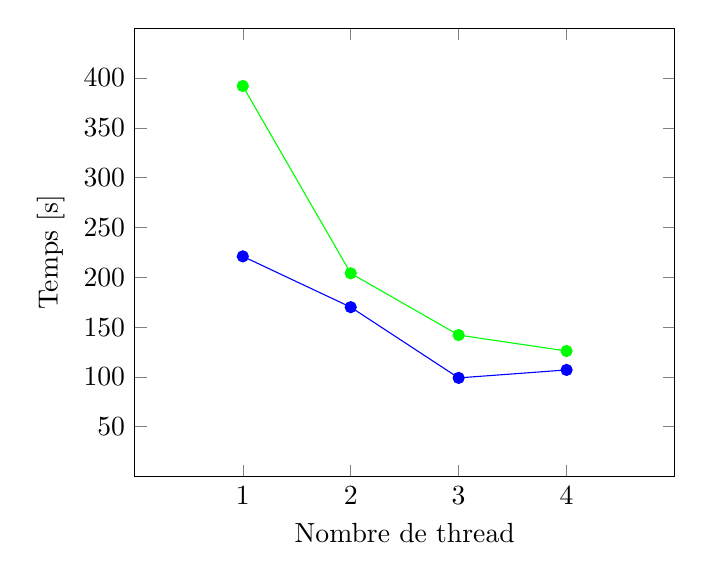
\begin{tikzpicture}
\begin{axis}[
xlabel={Nombre de thread},
ylabel={Temps [s]},
xmin=0,xmax=5,
ymin=0, ymax=450,
xtick={1,2,3,4},
ytick={50,100,150,200,250,300,350,400}]
\addplot[
color=blue,
mark=*,]
coordinates {
(1,221)(2,170)(3,99)(4,107)};
\addplot[
color=green,
mark=*,]
coordinates {
(1,392)(2,204)(3,142)(4,126)};
\end{axis}
\end{tikzpicture}
\caption{\label{graph1}Graphe des performances en fonction du nombre de thread}
\end{figure}
\subsection{Test sur des grands nombres}
Si les test sont exécutés sur des grands nombres, L'augmentation des performances est plus marqué car la factorisation prend comparativement aux autres fonctions plus de temps. C'est ce que montre la courbe verte du graphe \ref{graph1}. Le graphe montre que le temps décroit de manière exponentielle. La seule partie du temps qui diminue est le temps de la partie de factorisation des consommateur. Il reste toujours une partie du temps qui est utilisé pour publier les résultats dans la liste globale et l'analyse finale des résultats.\newpage
\subsection{Augmentation du nombre de nombre à factoriser}
L'analyse des performances en augmentant le nombre de nombre à factoriser montre que le temps de traitement dépend linéairement du nombre de nombre à traiter. 
\begin{figure}[!h]
\centering
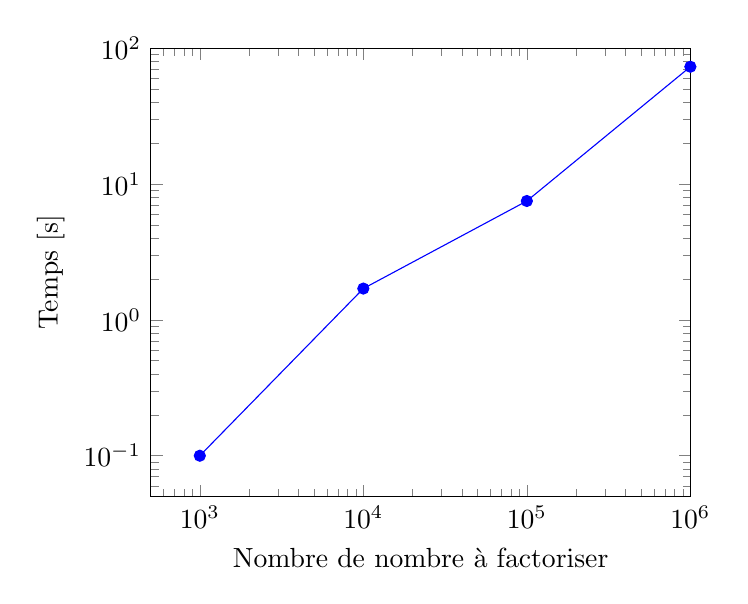
\begin{tikzpicture}
\begin{loglogaxis}[
xlabel={Nombre de nombre à factoriser},
ylabel={Temps [s]},
xmin=0,xmax=1e6,
ymin=0, ymax=100]
\addplot[color=blue,mark=*,]
coordinates{(1000,0.1)(10000,1.7)(100000,7.5)(1000000,73)};
\end{loglogaxis}
\end{tikzpicture}
\caption{\label{graph2}Graphe des performances en fonction de la taille de l'entrée}
\end{figure}
\end{document}